\documentclass[11pt,a4paper]{article}
\usepackage[utf8]{inputenc}
\usepackage{float,graphicx,amsfonts,amsmath,amssymb,authblk,graphicx,longtable,booktabs,fullpage}
\graphicspath{ {../img/} }
\usepackage[colorlinks = true,
            linkcolor = blue,
            urlcolor  = blue,
            citecolor = blue,
            anchorcolor = blue]{hyperref}
            

\title{Piano inclinato}

\author[1]{Dennis Angemi}%
\author[1]{Federica Ingrassia}%
\author[1]{Giuseppe Di Silvestre}%
\author[1]{Giulia De Luca}%
\affil[1]{Dipartimento di Fisica e Astronomia ``Ettore Majorana'' - Università degli Studi di Catania}%

\date{7 marzo 2022}

\begin{document}

\maketitle

\begin{abstract}
    L'obiettivo di questo studio è determinare il coefficiente di attrito di corpi tramite l'utilizzo di un piano inclinato.
\end{abstract}

\section{Introduzione e cenni teorici}
Il piano inclinato è un semplice dispositivo utilizzato in fisica per studiare le caratteristiche del moto uniformemente accelerato la cui prima descrizione si deve a Nicolas Oresme e a Galileo Galilei. Esso è costituito da una superficie piana disposta in modo da formare un angolo compreso tra 0° e 90° rispetto alla superficie orizzontale.

\begin{figure}[H]
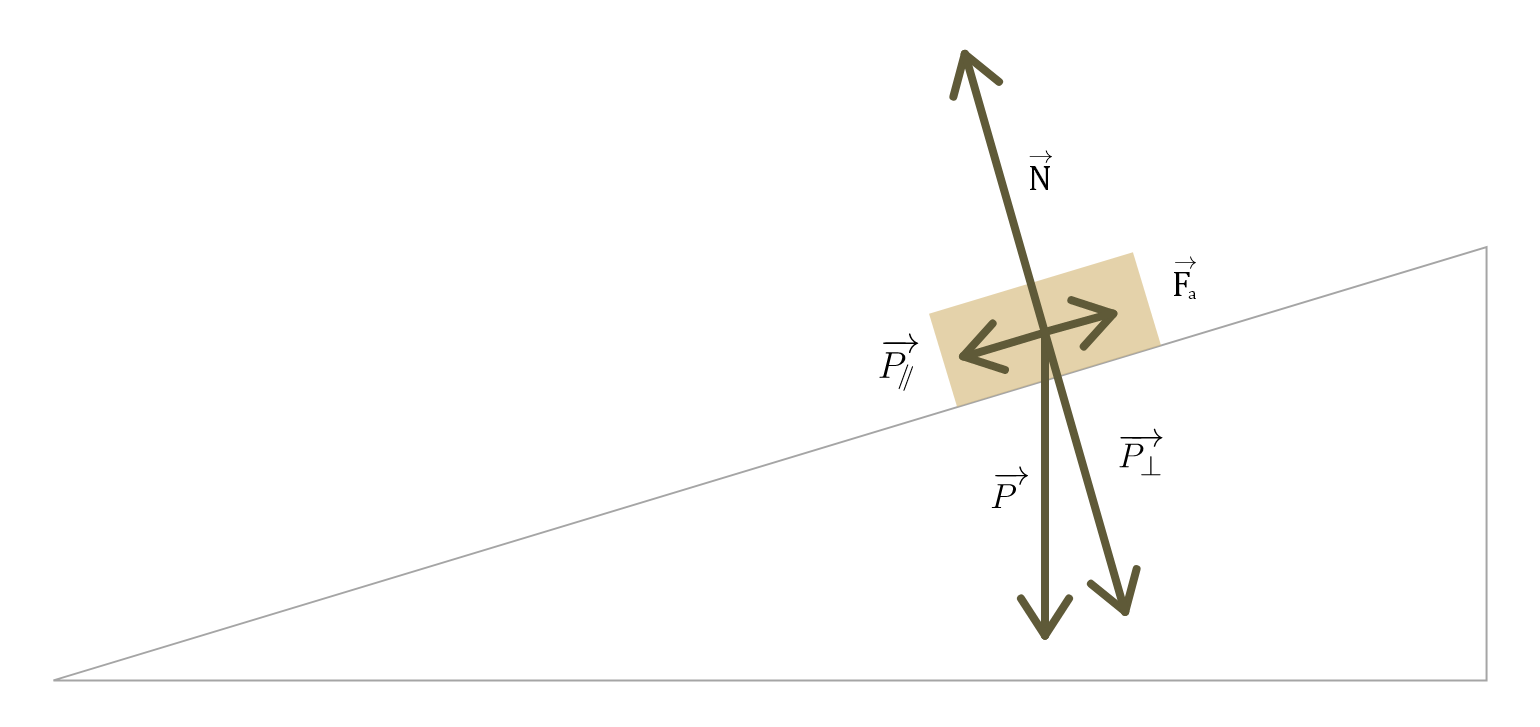
\includegraphics[scale=0.15]{force-diagram.png}
\centering
\caption{Diagramma delle forze}
\label{fig:forze}
\end{figure}

\section{Apparato sperimentale}

\subsection{Descrizione apparato}
L'apparato sperimentale è costituito da una guida d'acciaio dotata di una gola lungo la quale è possibile disporre diversi corpi con geometria differente in modo tale da permettere lo studio del modo di questi ultimi. Al di sopra della guida sono posizionate due fotocellule, disposte ad una distanza di 1.279 $\pm$ 0.002 m, collegate ad un timer digitale con sensibilità pari a 0.01 s.

\begin{figure}[H]
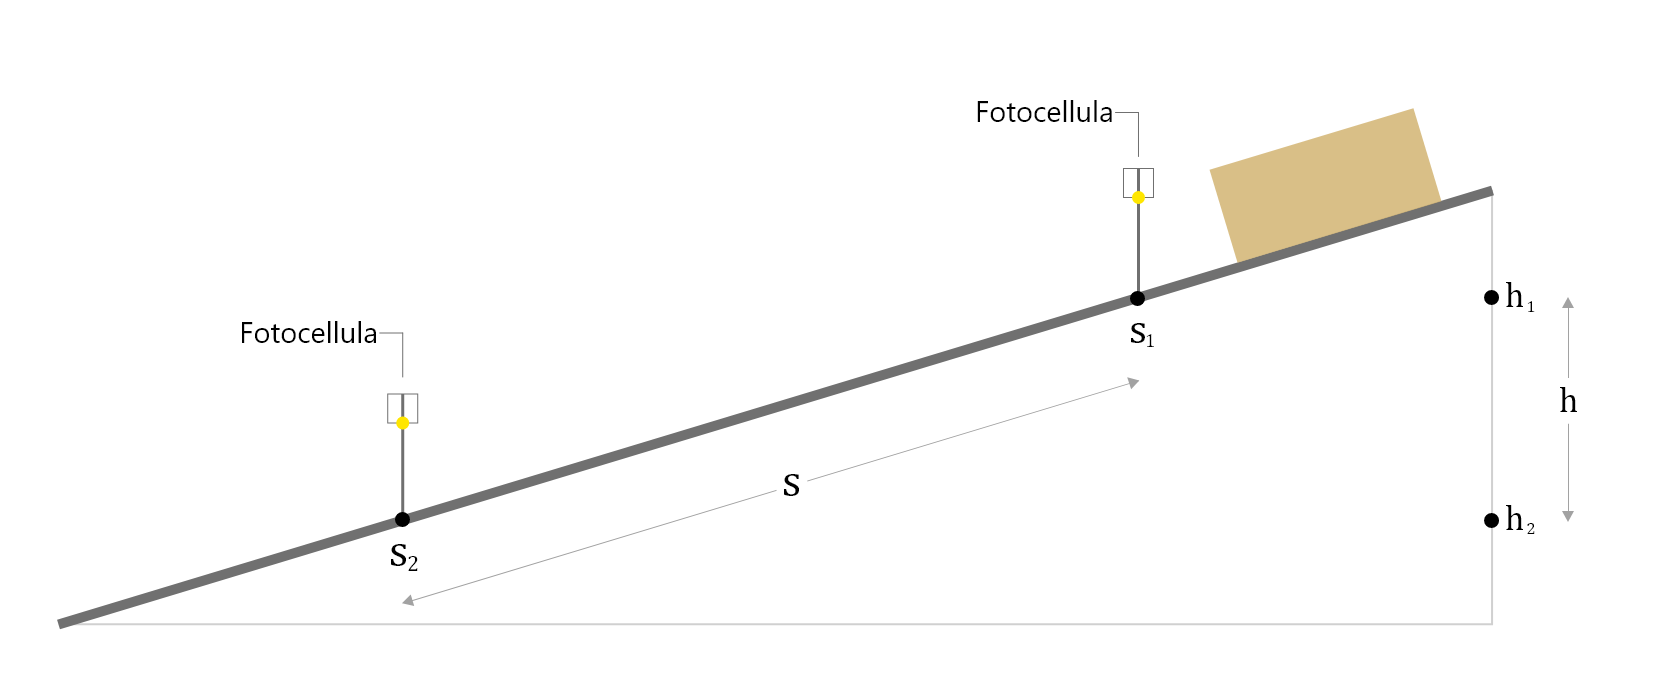
\includegraphics[scale=0.18]{experimental-setup.png}
\centering
\caption{Apparato sperimentale}
\label{fig:appspe}
\end{figure}

\subsection{Procedura di misura}
Per l'esperienza sono stati utilizzati 5 corpi differenti e per ognuno di essi sono state effettuate 40 misurazioni dell'intervallo di tempo impiegato da ciascun corpo per percorrere la distanza $\Delta s$. Le caratteristiche dei corpi utilizzati sono di seguito descritte:
\begin{itemize}
    \item $m_1$: cilindro di plastica
    \item $m_2$ ed $m_3$ cilindri di metallo
    \item $m_4$ sfera di metallo
    \item $m_5$ sfera di gomma
\end{itemize}

\begin{longtable}[]{@{}lllll@{}}
\toprule
Corpo & Massa\tabularnewline
\midrule
\endhead
$m_1$    & 15.19 $\pm$ 0.01 g  \tabularnewline
$m_2$    & 98.82 $\pm$ 0.01 g  \tabularnewline
$m_3$    & 130.60 $\pm$ 0.01 g \tabularnewline
$m_4$    & 13.79 $\pm$ 0.01 g  \tabularnewline
$m_5$    & 26.60 $\pm$ 0.01 g  \tabularnewline
\bottomrule
\end{longtable}

\subsection{Strumenti di misura}
I dati sperimentali sono stati ottenuti tramite l'utilizzo dei seguenti strumenti

\begin{longtable}[]{@{}lllll@{}}
\toprule
Strumento & Sensibilità & udm \tabularnewline
\midrule
\endhead
Flessometro & 0.001 & m \tabularnewline
Bilancia & 0.01 & g \tabularnewline
Cronometro & 0.01 & s \tabularnewline
\bottomrule
\end{longtable}


\section{Analisi dei dati e propagazione degli errori}
Al fine di ottenere il coefficiente di attrito tra il corpo m e la guida inclinata si utilizzano il secondo principio della dinamica e la legge oraria del moto rettilineo uniformemente accelerato con velocità iniziale nulla

\begin{equation}
    \begin{cases}
      mg \sin \theta - \mu mg \cos \theta = ma\\
      \Delta s=\frac{1}{2}a \Delta t^2 \\
    \end{cases}\
    \Longrightarrow
    \mu = \tan \theta - 2\frac{\Delta s}{\Delta t^2}\frac{1}{g \cos \theta}
\end{equation}



Avendo effettuato 40 misure dell'intervallo di tempo $\Delta t$ d'ora in poi utilizzeremo la seguente notazione

N=40

\begin{equation}
    \langle t \rangle = \frac{1}{N} \sum_{i=1}^N \Delta t_i
\end{equation}
    
\begin{equation}
    \mu = \tan \theta - 2\frac{\Delta s}{\langle t \rangle^2}\frac{1}{g \cos \theta}
\end{equation}

\subsection{Propagazione degli errori}
\begin{equation}
    \delta \mu = \left | \frac{\partial \mu}{\partial \theta} \right | \delta \theta + \left | \frac{\partial \mu}{\partial a} \right | \delta a + \left | \frac{\partial \mu}{\partial g} \right | \delta g
\end{equation}

attenzione: deltas è il doppio della sensibilità dello strumento

con 

\begin{equation}
    \delta a= \left | \frac{\partial a}{\partial s} \right | \delta s + \left | \frac{\partial a}{\partial \langle t \rangle ^2} \right | \delta \langle t \rangle ^2 = \frac{2}{\langle t \rangle ^2} (\delta s + 4s\delta t)
\end{equation}

\begin{equation}
    \delta \theta = \left | \frac{\partial \theta}{\partial t} \right | \delta t = 2 \delta s \left ( 1+\frac{h}{s} \right ) \frac{1}{\sqrt{s^2-h^2}}.
\end{equation}

In conclusione 
\begin{equation}
    \delta \mu = \frac{2\delta s}{\cos^2 \theta \sqrt{s^2-h^2}}\left ( 1- \frac{a \sin \theta}{g} \right ) \left ( 1+ \frac{h}{s}\right ) + \frac{2(\delta s + hs\delta t)}{\langle t \rangle ^2 g \cos \theta} + \frac{a \delta g}{g^2 \cos \theta}.
\end{equation}

\section{Risultati e conclusioni}

\begin{longtable}[]{@{}lllll@{}}
\toprule
Coefficiente di attrito & Errore assoluto & Errore relativo \tabularnewline
\midrule
\endhead
0.596 & 0.008 & 1.34 \% \tabularnewline
0.39 & 0.02 & 5.13 \% \tabularnewline
0.49 & 0.01 & 2.04 \% \tabularnewline
0.26 & 0.03 & 11.54 \% \tabularnewline
0.33 & 0.02 & 6.06 \% \tabularnewline
\bottomrule
\end{longtable}


\section{Additional notes}

\subsection{Data Availability}
The data that support the findings of this study are openly available in \href{https://github.com/dennisangemi/lab1-dfa/tree/main/exp-2/data}{dennisangemi/lab1-dfa GitHub Repository} at \href{https://github.com/dennisangemi/lab1-dfa/tree/main/exp-2/data}{https://github.com/dennisangemi/lab1-dfa/tree/main/exp-2/data} under \href{https://creativecommons.org/licenses/by/4.0/}{CC-BY 4.0 license}. Data are released with medatadata according to \href{https://frictionlessdata.io/standards/}{frictionless data standard.}

\subsection{Code Availability}
The MATLAB code written to get the findings of this study is openly available in \href{https://github.com/dennisangemi/lab1-dfa/tree/main/exp-2/script}{dennisangemi/lab1-dfa GitHub Repository} at \href{https://github.com/dennisangemi/lab1-dfa/tree/main/exp-2/script}{https://github.com/dennisangemi/lab1-dfa/tree/main/exp-2/script}


\subsection{Software used}
\begin{itemize}
\item
  \textbf{MATLAB}: Data Analysis
\item
  \textbf{Google Spreadsheet}: Data entry
\item
  \textbf{Adobe Experience Design}: Images designing
\item
  \textbf{GitHub}: Resource sharing
\end{itemize}

\section{Bibliography}
\begin{itemize}
\item
  Taylor,~ J. (1999).~\emph{Introduzione all'analisi degli errori: Lo
  studio delle incertezze nelle misure fisiche.~}Zanichelli
\item
  Bevington P. (2002).~\emph{Data Reduction and Error Analysis for the
  Physical Sciences.~} McGraw-Hill Education ~
\end{itemize}

\section{Appendice A}
\subsection{Tabella \ref{expdata1}}

\begin{longtable}[]{@{}lllll@{}}
%\caption{Dati sperimentali}
\toprule
Grandezza & Valore & Incertezza & udm \tabularnewline
\midrule
\endhead
$h_2$ & 0.412 & 0.001 & m \tabularnewline
$h_1$ & 1.122 & 0.001 & m \tabularnewline
$s_1$ & 1.992 & 0.001 & m \tabularnewline
$s_2$ & 0.713 & 0.001 & m \tabularnewline
$m_1$ & 15.19 & 0.01 & g \tabularnewline
$m_2$ & 98.82 & 0.01 & g \tabularnewline
$m_3$ & 130.60 & 0.01 & g \tabularnewline
$m_4$ & 13.79 & 0.01 & g \tabularnewline
$m_5$ & 26.60 & 0.01 & g \tabularnewline
\bottomrule
\label{expdata1}
\end{longtable}


\subsection{Tabella \ref{expdata2}}

\begin{longtable}[]{@{}lllll@{}}
\toprule
index & mass & t & uncertainty & uom \tabularnewline
\midrule
\endhead
1 & m1 & 1.65 & 0.01 & s \tabularnewline
2 & m1 & 1.60 & 0.01 & s \tabularnewline
3 & m1 & 1.66 & 0.01 & s \tabularnewline
4 & m1 & 2.18 & 0.01 & s \tabularnewline
5 & m1 & 1.54 & 0.01 & s \tabularnewline
6 & m1 & 1.74 & 0.01 & s \tabularnewline
7 & m1 & 1.47 & 0.01 & s \tabularnewline
8 & m1 & 1.55 & 0.01 & s \tabularnewline
9 & m1 & 1.80 & 0.01 & s \tabularnewline
10 & m1 & 1.75 & 0.01 & s \tabularnewline
11 & m1 & 1.94 & 0.01 & s \tabularnewline
12 & m1 & 2.05 & 0.01 & s \tabularnewline
13 & m1 & 2.67 & 0.01 & s \tabularnewline
14 & m1 & 1.56 & 0.01 & s \tabularnewline
15 & m1 & 2.45 & 0.01 & s \tabularnewline
16 & m1 & 1.43 & 0.01 & s \tabularnewline
17 & m1 & 2.08 & 0.01 & s \tabularnewline
18 & m1 & 2.02 & 0.01 & s \tabularnewline
19 & m1 & 1.55 & 0.01 & s \tabularnewline
20 & m1 & 1.88 & 0.01 & s \tabularnewline
21 & m1 & 2.31 & 0.01 & s \tabularnewline
22 & m1 & 1.67 & 0.01 & s \tabularnewline
23 & m1 & 1.72 & 0.01 & s \tabularnewline
24 & m1 & 2.37 & 0.01 & s \tabularnewline
25 & m1 & 1.60 & 0.01 & s \tabularnewline
26 & m1 & 1.44 & 0.01 & s \tabularnewline
27 & m1 & 1.69 & 0.01 & s \tabularnewline
28 & m1 & 2.50 & 0.01 & s \tabularnewline
29 & m1 & 2.15 & 0.01 & s \tabularnewline
30 & m1 & 1.48 & 0.01 & s \tabularnewline
31 & m1 & 1.17 & 0.01 & s \tabularnewline
32 & m1 & 1.51 & 0.01 & s \tabularnewline
33 & m1 & 1.24 & 0.01 & s \tabularnewline
34 & m1 & 1.44 & 0.01 & s \tabularnewline
35 & m1 & 1.73 & 0.01 & s \tabularnewline
36 & m1 & 1.37 & 0.01 & s \tabularnewline
37 & m1 & 1.49 & 0.01 & s \tabularnewline
38 & m1 & 1.34 & 0.01 & s \tabularnewline
39 & m1 & 1.31 & 0.01 & s \tabularnewline
40 & m1 & 1.39 & 0.01 & s \tabularnewline
1 & m2 & 0.98 & 0.01 & s \tabularnewline
2 & m2 & 0.87 & 0.01 & s \tabularnewline
3 & m2 & 0.92 & 0.01 & s \tabularnewline
4 & m2 & 0.95 & 0.01 & s \tabularnewline
5 & m2 & 0.93 & 0.01 & s \tabularnewline
6 & m2 & 0.91 & 0.01 & s \tabularnewline
7 & m2 & 0.85 & 0.01 & s \tabularnewline
8 & m2 & 0.89 & 0.01 & s \tabularnewline
9 & m2 & 0.86 & 0.01 & s \tabularnewline
10 & m2 & 0.86 & 0.01 & s \tabularnewline
11 & m2 & 1.00 & 0.01 & s \tabularnewline
12 & m2 & 0.92 & 0.01 & s \tabularnewline
13 & m2 & 0.89 & 0.01 & s \tabularnewline
14 & m2 & 0.93 & 0.01 & s \tabularnewline
15 & m2 & 0.87 & 0.01 & s \tabularnewline
16 & m2 & 0.87 & 0.01 & s \tabularnewline
17 & m2 & 0.89 & 0.01 & s \tabularnewline
18 & m2 & 0.87 & 0.01 & s \tabularnewline
19 & m2 & 0.87 & 0.01 & s \tabularnewline
20 & m2 & 0.94 & 0.01 & s \tabularnewline
21 & m2 & 0.91 & 0.01 & s \tabularnewline
22 & m2 & 0.86 & 0.01 & s \tabularnewline
23 & m2 & 0.93 & 0.01 & s \tabularnewline
24 & m2 & 0.87 & 0.01 & s \tabularnewline
25 & m2 & 0.93 & 0.01 & s \tabularnewline
26 & m2 & 0.87 & 0.01 & s \tabularnewline
27 & m2 & 0.54 & 0.01 & s \tabularnewline
28 & m2 & 0.88 & 0.01 & s \tabularnewline
29 & m2 & 0.84 & 0.01 & s \tabularnewline
30 & m2 & 0.94 & 0.01 & s \tabularnewline
31 & m2 & 0.99 & 0.01 & s \tabularnewline
32 & m2 & 0.89 & 0.01 & s \tabularnewline
33 & m2 & 0.90 & 0.01 & s \tabularnewline
34 & m2 & 0.91 & 0.01 & s \tabularnewline
35 & m2 & 0.86 & 0.01 & s \tabularnewline
36 & m2 & 0.88 & 0.01 & s \tabularnewline
37 & m2 & 0.91 & 0.01 & s \tabularnewline
38 & m2 & 0.81 & 0.01 & s \tabularnewline
39 & m2 & 0.92 & 0.01 & s \tabularnewline
40 & m2 & 0.88 & 0.01 & s \tabularnewline
1 & m3 & 1.45 & 0.01 & s \tabularnewline
2 & m3 & 1.21 & 0.01 & s \tabularnewline
3 & m3 & 1.33 & 0.01 & s \tabularnewline
4 & m3 & 1.19 & 0.01 & s \tabularnewline
5 & m3 & 1.12 & 0.01 & s \tabularnewline
6 & m3 & 1.03 & 0.01 & s \tabularnewline
7 & m3 & 1.23 & 0.01 & s \tabularnewline
8 & m3 & 1.25 & 0.01 & s \tabularnewline
9 & m3 & 1.13 & 0.01 & s \tabularnewline
10 & m3 & 1.13 & 0.01 & s \tabularnewline
11 & m3 & 1.07 & 0.01 & s \tabularnewline
12 & m3 & 1.15 & 0.01 & s \tabularnewline
13 & m3 & 1.14 & 0.01 & s \tabularnewline
14 & m3 & 1.05 & 0.01 & s \tabularnewline
15 & m3 & 1.08 & 0.01 & s \tabularnewline
16 & m3 & 1.10 & 0.01 & s \tabularnewline
17 & m3 & 1.02 & 0.01 & s \tabularnewline
18 & m3 & 1.07 & 0.01 & s \tabularnewline
19 & m3 & 1.04 & 0.01 & s \tabularnewline
20 & m3 & 1.05 & 0.01 & s \tabularnewline
21 & m3 & 1.01 & 0.01 & s \tabularnewline
22 & m3 & 1.02 & 0.01 & s \tabularnewline
23 & m3 & 1.07 & 0.01 & s \tabularnewline
24 & m3 & 1.07 & 0.01 & s \tabularnewline
25 & m3 & 1.02 & 0.01 & s \tabularnewline
26 & m3 & 0.99 & 0.01 & s \tabularnewline
27 & m3 & 1.03 & 0.01 & s \tabularnewline
28 & m3 & 1.03 & 0.01 & s \tabularnewline
29 & m3 & 1.10 & 0.01 & s \tabularnewline
30 & m3 & 1.01 & 0.01 & s \tabularnewline
31 & m3 & 1.10 & 0.01 & s \tabularnewline
32 & m3 & 1.21 & 0.01 & s \tabularnewline
33 & m3 & 1.05 & 0.01 & s \tabularnewline
34 & m3 & 1.07 & 0.01 & s \tabularnewline
35 & m3 & 1.11 & 0.01 & s \tabularnewline
36 & m3 & 1.03 & 0.01 & s \tabularnewline
37 & m3 & 1.07 & 0.01 & s \tabularnewline
38 & m3 & 1.04 & 0.01 & s \tabularnewline
39 & m3 & 1.06 & 0.01 & s \tabularnewline
40 & m3 & 1.11 & 0.01 & s \tabularnewline
1 & m4 & 0.73 & 0.01 & s \tabularnewline
2 & m4 & 0.75 & 0.01 & s \tabularnewline
3 & m4 & 0.74 & 0.01 & s \tabularnewline
4 & m4 & 0.73 & 0.01 & s \tabularnewline
5 & m4 & 0.73 & 0.01 & s \tabularnewline
6 & m4 & 0.72 & 0.01 & s \tabularnewline
7 & m4 & 0.73 & 0.01 & s \tabularnewline
8 & m4 & 0.74 & 0.01 & s \tabularnewline
9 & m4 & 0.73 & 0.01 & s \tabularnewline
10 & m4 & 0.73 & 0.01 & s \tabularnewline
11 & m4 & 0.73 & 0.01 & s \tabularnewline
12 & m4 & 0.73 & 0.01 & s \tabularnewline
13 & m4 & 0.73 & 0.01 & s \tabularnewline
14 & m4 & 0.71 & 0.01 & s \tabularnewline
15 & m4 & 0.72 & 0.01 & s \tabularnewline
16 & m4 & 0.73 & 0.01 & s \tabularnewline
17 & m4 & 0.72 & 0.01 & s \tabularnewline
18 & m4 & 0.72 & 0.01 & s \tabularnewline
19 & m4 & 0.72 & 0.01 & s \tabularnewline
20 & m4 & 0.71 & 0.01 & s \tabularnewline
21 & m4 & 0.71 & 0.01 & s \tabularnewline
22 & m4 & 0.71 & 0.01 & s \tabularnewline
23 & m4 & 0.72 & 0.01 & s \tabularnewline
24 & m4 & 0.73 & 0.01 & s \tabularnewline
25 & m4 & 0.73 & 0.01 & s \tabularnewline
26 & m4 & 0.72 & 0.01 & s \tabularnewline
27 & m4 & 0.73 & 0.01 & s \tabularnewline
28 & m4 & 0.73 & 0.01 & s \tabularnewline
29 & m4 & 0.73 & 0.01 & s \tabularnewline
30 & m4 & 0.72 & 0.01 & s \tabularnewline
31 & m4 & 0.74 & 0.01 & s \tabularnewline
32 & m4 & 0.72 & 0.01 & s \tabularnewline
33 & m4 & 0.74 & 0.01 & s \tabularnewline
34 & m4 & 0.73 & 0.01 & s \tabularnewline
35 & m4 & 0.73 & 0.01 & s \tabularnewline
36 & m4 & 0.74 & 0.01 & s \tabularnewline
37 & m4 & 0.73 & 0.01 & s \tabularnewline
38 & m4 & 0.73 & 0.01 & s \tabularnewline
39 & m4 & 0.72 & 0.01 & s \tabularnewline
40 & m4 & 0.74 & 0.01 & s \tabularnewline
1 & m5 & 0.80 & 0.01 & s \tabularnewline
2 & m5 & 0.80 & 0.01 & s \tabularnewline
3 & m5 & 0.79 & 0.01 & s \tabularnewline
4 & m5 & 0.80 & 0.01 & s \tabularnewline
5 & m5 & 0.80 & 0.01 & s \tabularnewline
6 & m5 & 0.81 & 0.01 & s \tabularnewline
7 & m5 & 0.81 & 0.01 & s \tabularnewline
8 & m5 & 0.81 & 0.01 & s \tabularnewline
9 & m5 & 0.80 & 0.01 & s \tabularnewline
10 & m5 & 0.82 & 0.01 & s \tabularnewline
11 & m5 & 0.80 & 0.01 & s \tabularnewline
12 & m5 & 0.79 & 0.01 & s \tabularnewline
13 & m5 & 0.81 & 0.01 & s \tabularnewline
14 & m5 & 0.82 & 0.01 & s \tabularnewline
15 & m5 & 0.80 & 0.01 & s \tabularnewline
16 & m5 & 0.73 & 0.01 & s \tabularnewline
17 & m5 & 0.80 & 0.01 & s \tabularnewline
18 & m5 & 0.81 & 0.01 & s \tabularnewline
19 & m5 & 0.82 & 0.01 & s \tabularnewline
20 & m5 & 0.79 & 0.01 & s \tabularnewline
21 & m5 & 0.79 & 0.01 & s \tabularnewline
22 & m5 & 0.80 & 0.01 & s \tabularnewline
23 & m5 & 0.81 & 0.01 & s \tabularnewline
24 & m5 & 0.82 & 0.01 & s \tabularnewline
25 & m5 & 0.82 & 0.01 & s \tabularnewline
26 & m5 & 0.80 & 0.01 & s \tabularnewline
27 & m5 & 0.82 & 0.01 & s \tabularnewline
28 & m5 & 0.81 & 0.01 & s \tabularnewline
29 & m5 & 0.81 & 0.01 & s \tabularnewline
30 & m5 & 0.83 & 0.01 & s \tabularnewline
31 & m5 & 0.82 & 0.01 & s \tabularnewline
32 & m5 & 0.81 & 0.01 & s \tabularnewline
33 & m5 & 0.80 & 0.01 & s \tabularnewline
34 & m5 & 0.80 & 0.01 & s \tabularnewline
35 & m5 & 0.80 & 0.01 & s \tabularnewline
36 & m5 & 0.80 & 0.01 & s \tabularnewline
37 & m5 & 0.81 & 0.01 & s \tabularnewline
38 & m5 & 0.81 & 0.01 & s \tabularnewline
39 & m5 & 0.81 & 0.01 & s \tabularnewline
40 & m5 & 0.80 & 0.01 & s \tabularnewline
\bottomrule
\label{expdata2}
\end{longtable}

\end{document}
